\iffalse
\documentclass[journal,12pt,twocolumn]{IEEEtran}
\usepackage{amsmath,amssymb,amsfonts,amsthm}
\usepackage{txfonts}
\usepackage{tkz-euclide}
\usepackage{listings}
\usepackage{gvv}
\usepackage[latin1]{inputenc}
\usepackage{adjustbox}
\usepackage{array}
\usepackage{tabularx}
\usepackage{enumitem}
\usepackage{pgf}
\usepackage{lmodern}
\usepackage{circuitikz}
\usepackage{tikz}
\usepackage{graphicx}


\begin{document}
\bibliographystyle{IEEEtran}

\vspace{3cm}

\title{}
\author{EE23BTECH11054 -  Sai Krishna Shanigarapu$^{*}$
}
\maketitle
\newpage
\bigskip

% \renewcommand{\thefigure}{\theenumi}
% \renewcommand{\thetable}{\theenumi}

\section*{Gate EC 2022}
54. \hspace{2pt}In a circuit, there is a series connection of an ideal resistor and an ideal capacitor.
The conduction current (in Amperes) through the resistor is $2\sin\brak{t + \frac{\pi}{2}}$. The displacement current (in Amperes) through the capacitor is \rule{1cm}{0.15mm}.\\ 
\begin{enumerate}[label=(\Alph*)]
    \item $2\sin\brak{t}$
    \item $2\sin\brak{t+\pi}$
    \item $2\sin\brak{t +\frac{\pi}{2}}$
    \item $0$
\end{enumerate}
\hfill(GATE EC 2022)

\solution
\fi
\begin{table}[ht]
       \setlength{\arrayrulewidth}{0.3mm}
\setlength{\tabcolsep}{20pt}
\renewcommand{\arraystretch}{1.5}

\begin{tabular}{|c|c|c|}
\hline
Parameter& Description & Value\\
\hline
$I_c$ & Conduction Current & $2\sin\brak{t + \frac{\pi}{2}}$\\
\hline
%$I_d$ & Displacement current & ?\\
%\hline
$A$ & Cross-sectional area & \\
\hline
\end{tabular}

    \caption{Parameters}
    \label{tab:tab_gate_ec_2022_24_1}
\end{table}


\begin{table}[ht]
       \setlength{\arrayrulewidth}{0.3mm}
\setlength{\tabcolsep}{20pt}
\renewcommand{\arraystretch}{1.5}

\begin{tabular}{|c|c|c|}
\hline
Parameter & Description & Formula\\
\hline
$Q$ & Charge & $\int I_c\, dt$\\
\hline
$D$ & Electric Displacement & $\frac{Q}{A}$\\ 
\hline
$J_D$ & Displacement current density & $\frac{\partial D}{\partial t}$\\
\hline
$I_D$ & Displacement current & $J_D\text{ x }A$\\
\hline




\end{tabular}

    \caption{Formulae}
    \label{tab:tab_gate_ec_2022_24_2}
\end{table}

\begin{table}[ht]
       \setlength{\arrayrulewidth}{0.3mm}
\setlength{\tabcolsep}{20pt}
\renewcommand{\arraystretch}{1.5}



\begin{tabular}{|c|c|}
\hline

S Domain & Time Domain\\
\hline
$\frac{1}{s}$ & $u\brak{t}$\\
\hline
$\frac{-s}{a^2+s^2}$ & $-\cos\brak{at}$\\
\hline
$\frac{a}{a^2+s^2}$ & $\sin\brak{at}$\\
\hline
$\frac{1}{s+a}$ & $e^{-at}$\\
\hline

\end{tabular}


    \caption{Laplace transforms}
    \label{tab:tab_gate_ec_2022_24_3}
\end{table}

\begin{align}
    \mathcal{L}\sbrak{\int f\brak{t}\, dt} &= \int_{0}^{\infty}\sbrak{\int f\brak{t}\, dt}e^{-st}\, dt\\
    &= \int_{0}^{\infty}u\, dv \quad \text{where}\begin{cases}
  u =\int f\brak{t}dt \\
  dv  =e^{-st}dt
\end{cases}\\
&= uv - v\int du\\
&= \frac{1}{s}\int f\brak{t}dt|_0 + \frac{1}{s}\int_{0}^{\infty}f\brak{t}e^{-st}dt\\
&\implies \frac{1}{s}\int f\brak{t}dt|_0 + \frac{1}{s}F\brak{s} \label{eq:eq_gate_ec_2022_24_1}
\end{align}


\begin{figure}[ht]
  \centering
      \begin{circuitikz}[american]
\draw (0,3) to [short,*-, i=$i_c$] (1,3) to [R=$R$] (4,3);
\draw (0,0) to [short, *-] (4,0);
\draw (4,3) to [short, i=$i_d$] (4,2.5) to [C=$C$] (4,0);
\end{circuitikz}
  \caption{Circuit 1}
\end{figure}

From Table \ref{tab:tab_gate_ec_2022_24_2}, Table \ref{tab:tab_gate_ec_2022_24_3} and eq (\ref{eq:eq_gate_ec_2022_24_1})
\begin{align}
    I_c\brak{s} &= \frac{2s}{s^2 + 1}\\
    Q_c\brak{s} &= \frac{2}{s\brak{s^2 + 1}}\\
    D\brak{s} &= \frac{1}{A}\brak{\frac{2}{s\brak{s^2 + 1}}}\\
    J_D\brak{s} &= \frac{2}{A}\brak{\frac{1}{s^2 + 1}}\\
    I_D\brak{s} &= \frac{2}{s^2 + 1}\\
    \implies I_D &= 2\sin{t}
\end{align}


\begin{figure}[ht]
  \centering
      \begin{tikzpicture}

        \draw[->] (-0.5,0) -- (4.5,0) node[right]{$E_{\text{ref}}$};
        \draw[->] (0,-0.5) -- (0,4.5) node[above]{$J_d$};
        

        \draw (0,0) -- (4,4);
        

        \draw[dashed] (4,0) -- (4,4);
        \node[right] at (4,4) {$\overline{J}$};
        \draw[dotted] (4,4) -- (4,0) node[below]{$J_c$};

        \draw[dashed] (0,4) -- (4,4);
        \draw[dotted] (4,4) -- (0,4) node[left]{$J_d$};
        

        \draw[->] (0.5,0) arc (0:90:0.5);
        \node[right] at (0.5,0.3) {$\frac{\pi}{2}$};
\end{tikzpicture}


  \caption{Phasor plot}
  \label{fig:fig_gate_ec_2022_24_1}
\end{figure}

From figure \ref{fig:fig_gate_ec_2022_24_1}, phase of $I_d$ is $\frac{\pi}{2}$

\begin{align}
    \therefore I_d = 2\sin\brak{t + \frac{\pi}{2}}
\end{align}
$\therefore$ (C) is correct.


\begin{figure}[ht]
    \centering
    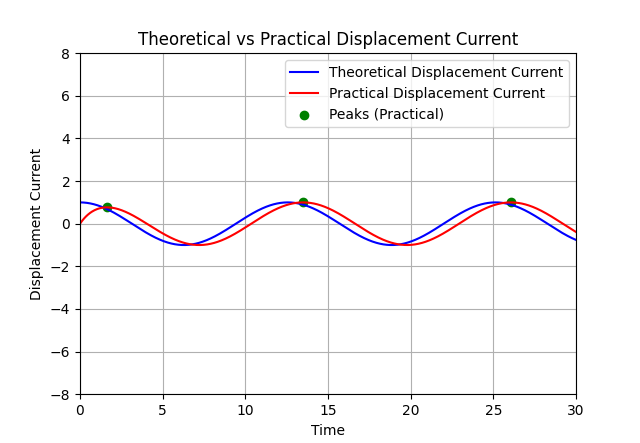
\includegraphics[width=\columnwidth]{2022/EC/24/figs/Figure_2.png}
    \caption{Thoritical vs Practical simulation}
    \label{fig:fig_gate_ec_2022_24_2}
\end{figure}

\begin{figure}[ht]
    \centering
    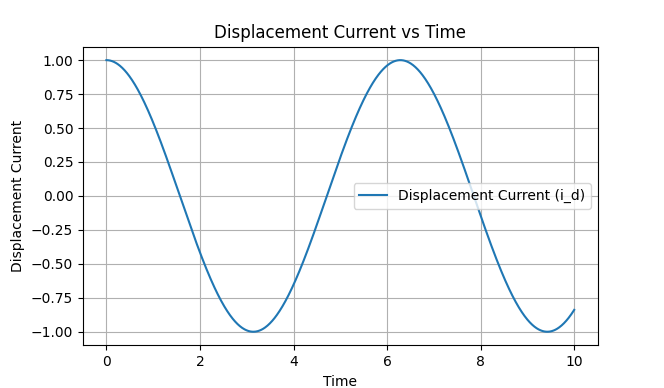
\includegraphics[width=\columnwidth]{2022/EC/24/figs/Figure_4.png}
    \caption{Displacement current}
    \label{fig:fig_gate_ec_2022_24_3}
\end{figure}



%\end{document}
